% !TEX program = xelatex
% Mixed raster/vector. Source: locked Jan20 2022 author PDF, pp11-14/S3/S5/S6.
% Generated viewports supply illustrations only; equations/arrows are independently checked.
\documentclass[tikz,border=2mm]{standalone}
\usepackage{fontspec,xeCJK,amsmath,amssymb,graphicx}
\setsansfont{Arial}
\setCJKmainfont[Path=/System/Library/Fonts/,BoldFont={STHeiti Medium.ttc}]{STHeiti Light.ttc}
\setCJKsansfont[Path=/System/Library/Fonts/,BoldFont={STHeiti Medium.ttc}]{STHeiti Light.ttc}
\renewcommand{\familydefault}{\sfdefault}
\usetikzlibrary{arrows.meta,calc}
\definecolor{ink}{HTML}{173646}
\definecolor{teal}{HTML}{217E80}
\definecolor{amber}{HTML}{B5712F}
\definecolor{purple}{HTML}{735098}
\definecolor{pale}{HTML}{F6F8F7}
\definecolor{warm}{HTML}{FFF6E9}
\definecolor{violet}{HTML}{F3EFF9}
\tikzset{t/.style={text=ink,font=\fontsize{16.5}{20}\selectfont,align=center,inner sep=0},
 hd/.style={t,font=\bfseries\fontsize{21}{25}\selectfont},
 sm/.style={t,font=\fontsize{15}{18}\selectfont},
 a/.style={-{Stealth[length=3mm,width=2mm]},line width=1.4pt,draw=teal,rounded corners=2pt},
 sup/.style={a,draw=amber,dashed},
 box/.style={rounded corners=4pt,line width=.8pt}}
\newcommand{\txt}[4]{\node[t,text width=#3cm]at(#1,#2){#4};}
\newcommand{\head}[4]{\node[hd,text width=#3cm]at(#1,#2){#4};}
\newcommand{\smalltxt}[4]{\node[sm,text width=#3cm]at(#1,#2){#4};}
\newcommand{\maths}[4]{\node[text=ink,font=\fontsize{#3}{#3}\selectfont,inner sep=0]at(#1,#2){\(\displaystyle #4\)};}
\newcommand{\panel}[7]{\draw[box,draw=#6!45,fill=#7](#1,#2)rectangle++(#3,#4);\pgfmathsetmacro{\pw}{#3-.3}\head{#1+#3/2}{#2+.47}{\pw}{#5}}
% Source PNG has 1536x1024 pixels and 72dpi natural size. Unmodified viewports.
\newcommand{\art}[7]{\begingroup\pgfmathsetmacro{\bt}{1024-#2-#4}\pgfmathsetmacro{\rt}{1536-#1-#3}
\node[anchor=north west,inner sep=0]at(#5,#6){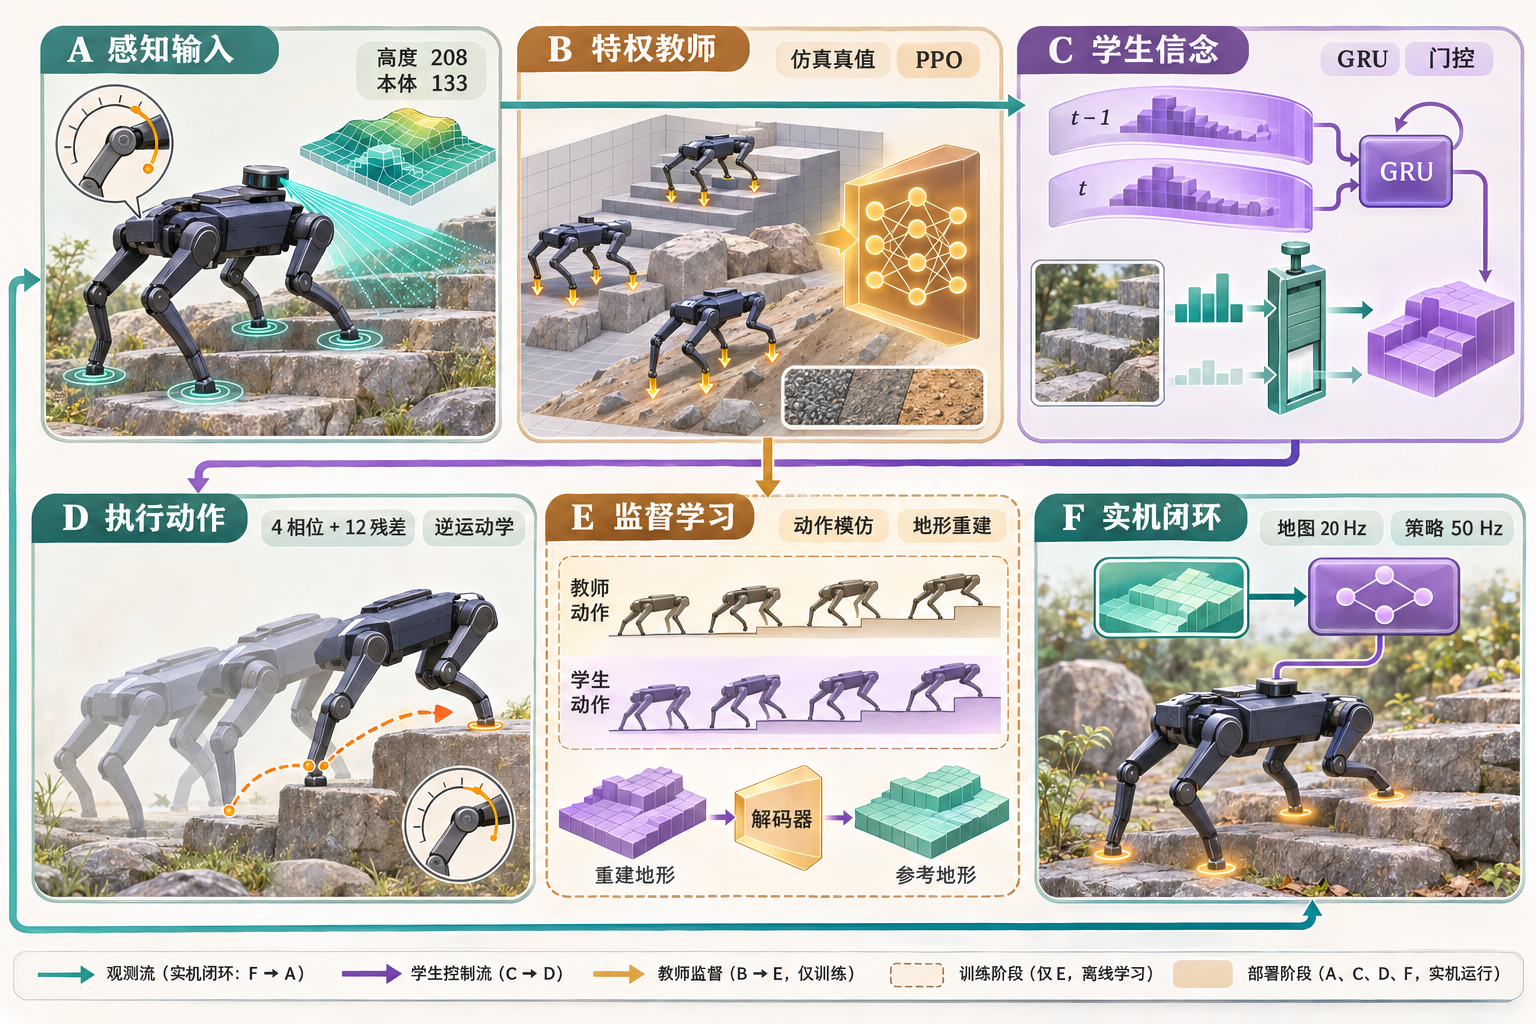
\includegraphics[trim=#1bp \bt bp \rt bp #2bp,clip,width=#7cm]{perceptive-loco-imagegen-draft.png}};\endgroup}
\begin{document}
\begin{tikzpicture}[x=1cm,y=-1cm]
\path[use as bounding box](0,0)rectangle(18,28.2);\fill[white](0,0)rectangle(18,28.2);
\head{9}{.45}{17.2}{机器狗怎样决定：眼前地形该信几分？}
\smalltxt{9}{1.03}{17}{青色实线：运行数据\qquad 暖色虚线：训练监督}
\panel{.85}{1.55}{7.7}{7.25}{A\quad 感知输入}{teal}{pale}
\begin{scope}\clip(1.4,2.35)--(5.8,2.35)--(5.8,2.72)--(8,2.72)--(8,7.47)--(1.4,7.47)--cycle;\art{42}{82}{457}{354}{1.4}{2.35}{6.6}\end{scope}
\txt{4.7}{7.93}{7.2}{四脚高度样本 208}
\txt{4.7}{8.49}{7.2}{本体与速度指令 133}
\panel{9.45}{1.55}{7.7}{7.25}{B\quad 特权教师}{amber}{warm}
\art{523}{113}{464}{320}{9.85}{2.35}{6.9}
\txt{13.3}{7.52}{7.2}{干净高度 + 仿真特权}
\txt{13.3}{8.13}{7.2}{PPO 学出 16 维动作}
\panel{.85}{9.6}{7.7}{8.3}{C\quad 学生信念}{purple}{violet}
\art{1048}{86}{289}{144}{1.13}{10.45}{4.3}
\art{1173}{241}{164}{168}{5.7}{10.6}{2.2}
\txt{4.7}{13.08}{7.1}{本体 + 高度 + 历史}
\txt{4.7}{13.77}{7.1}{GRU：2 层，每层 50}
\maths{4.7}{14.55}{17}{\alpha_t=\sigma(g_a(b'_t))\in(0,1)^{96}}
\txt{4.7}{15.3}{7.0}{96 维高度特征逐项门控}
\txt{4.7}{16.02}{7.0}{补零，加入 120 维信念}
\smalltxt{4.7}{16.7}{7.0}{高度特征仍进入 GRU}\smalltxt{4.7}{17.35}{7.0}{本体 + 信念 → 动作 MLP}
\panel{9.45}{9.6}{7.7}{8.3}{E\quad 学生训练}{amber}{warm}
\art{559}{556}{449}{192}{9.85}{10.45}{6.9}
\txt{13.3}{13.79}{7.0}{学生走，教师给动作标签}
\txt{13.3}{14.58}{7.0}{隐藏状态 + 带噪高度}
\txt{13.3}{15.32}{7.0}{解码：208 高度 + 50 特权}
\maths{13.3}{16.12}{19}{\mathcal L=\mathcal L_{bc}+0.5\mathcal L_{re}}
\smalltxt{13.3}{16.93}{7.0}{教师固定，双损失更新学生}
\panel{.85}{18.7}{7.7}{7.6}{D\quad 从动作到关节}{teal}{pale}
\art{46}{558}{482}{335}{1.25}{19.5}{6.9}
\txt{4.7}{24.68}{7.1}{4 相位 + 12 关节残差}
\txt{4.7}{25.34}{7.1}{轨迹 → IK → 12 目标角}
\panel{9.45}{18.7}{7.7}{7.6}{F\quad 实机闭环}{teal}{pale}
\art{1040}{558}{470}{337}{10.65}{19.5}{5.3}
\txt{13.3}{23.65}{7.0}{地图 20 Hz；策略 50 Hz}
\txt{13.3}{24.43}{7.0}{参数固定，隐藏状态更新}
\txt{13.3}{25.21}{7.0}{新观测进入下一步}
\draw[a](4.7,8.8)--(4.7,9.6);
\draw[a](4.7,17.9)--(4.7,18.7);
\draw[a](8.55,22.5)--(9.45,22.5);
\draw[sup](13.3,8.8)--(13.3,9.6);
\draw[sup](9.45,15.8)--(8.55,15.8);
\draw[a](13.3,26.3)--(13.3,27.1)--(.35,27.1)--(.35,5.7)--(.85,5.7);
\smalltxt{9}{27.7}{16.9}{训练：B → E → C\qquad 运行：A → C → D → F → A}
\end{tikzpicture}
\end{document}
